% ==== 原文 p.28 ====
\subsection{带源的量子化}\label{sec:4.2}
% 原文标题：4.2 Quantization with Sources

\paragraph{插入威尔逊圈}
我们现已准备好做一件真正有物理意义的事：描述有物质存在时 CS 理论的希尔伯特空间结构。等价地，正如 \S\ref{sec:2.2} 中所见，只要考虑存在威尔逊圈的理论，我们就能把 $\SCS$ 与源耦合起来。图 \ref{fig:cut} 示意了这一点。它提示：一个威尔逊圈在 $\Sigma$ 上留下的印记，是一组静态的非阿贝尔电荷。在 $A_0=0$ 规范下，设 $\Sigma$ 上的点 $p_1,\dots,p_r$ 处有 $r$ 个这样的电荷，则 CS 理论的高斯定律成为
\begin{equation}\tag{4.5}\label{eq:4.5}
  \frac{k}{4\pi}\varepsilon^{ij}F^{a}_{ij} = \sum_{s=1}^{r}\delta^{(2)}(x-p_s)T^{a}_{s}.
\end{equation}
这里 $T^{a}_{s}\in\mathfrak{g}$ 是分配给每个电荷的李代数生成元。在量子理论中，这些生成元应按相应的表示 $R_s$ 来理解。

% [Tutor Note: 易错点] (4.5) 左端的 k/4π 来自 S_CS 对 A_0 的变分，与 (4.2) 的 2π/k 角色不同、不可互换；ε^{ij} 与 ε_{ij} 的上下标、δ^(2) 的密度性质都须留意。
\begin{yizhu}[易错点]
(4.5) 左端的 $k/4\pi$ 来自 $\SCS$ 对 $A_0$ 的变分，不要与 \eqref{eq:4.2} 的 $2\pi/k$ 混用：后者是辛形式（泊松括号）的归一化，前者是约束方程的系数，两者出自同一个 $\SCS$ 却各司其职。又因 $\varepsilon^{ij}F_{ij}=2\varepsilon^{ij}\partial_iA_j$ 带因子 $2$，两个系数相乘只给出 $1/2$ 而不是 $1$，不能靠「互逆」来记忆。指标上，左端用 $\varepsilon^{ij}$，\eqref{eq:4.2} 用 $\varepsilon_{ij}$：在平坦 $\R^2$ 上二者数值相同，搬到弯曲 $\Sigma$ 上须换成面积形式，$\delta^{(2)}$ 也应按密度理解。
\end{yizhu}

% [Tutor Note: 易错点] T^a_s 在 (4.5) 里是李代数元，在量子理论里是表示 R_s 中的算子；反厄米性使 iT^a_s 才是可观测量，这是后文「去量子化」的依据。
\begin{yizhu}[易错点]
$T^{a}_{s}$ 在两处含义不同。在 (4.5) 这个经典约束里，它是 $\mathfrak{g}$ 中为每个电荷选定的生成元；进入量子理论后，它必须读作表示 $R_s$ 中的算子 $T^{a}(R_s)$，每个标记点带自己的表示。因此 (4.5) 的右端是算符值分布，不同 $s$ 的 $T^{a}_{s}$ 作用在各自的表示上，严格说要先写进张量积 $R_1\otimes\cdots\otimes R_r$ 再谈相加。作者另点明 $T^{a}_{s}$ 反厄米，故 $iT^{a}_{s}$ 才是可观测量——这正是后文能把 $T^{a}_{s}$ 换成相空间函数的依据。
\end{yizhu}

\paragraph{如何「不」量子化}
% 原文标题：How \emph{not} to quantize.
(4.5) 的量子化看上去是件令人望而生畏的任务。朴素的做法是先量子化泊松括号 \eqref{eq:4.2}，再在量子层面施加带源的高斯定律；这个做法比无源情形更加不切实际。在经典层面施加约束似乎是唯一的出路，但即便如此也会立刻撞上困难：其一，由 (4.5) 定义的联络绝对不是平坦的。这时已看不出如何在经典解空间上安放辛结构；更一般地，平坦性的失效会使我们几何机器的一大片随之崩坏。更令人担忧的是，(4.5) 中出现的生成元 $T^a$ 并不对易。于是它们定义的「联络」不可能是普通的主联络，只能是某种古怪的非对易对象。这些思量恰好是非交换几何与量子群理论 [25] 的自然起点，二者都对上述问题给出了自然的表述与解法。不过我们不打算沿这条路线走。我们换一个更洒脱的视角：注意 (4.5) 所定义的联络其实\textbf{是}平坦的，只在标记点 $p_1,\dots,p_r$ 处例外——那里它带有非阿贝尔的 delta 函数「缺陷」。我们可以合理地指望：一旦学会处理这些静态电荷，或许就能以某种方式修改或扩充平坦联络的模空间，把它们的效应纳入其中。为此，我们需要绕一小段路。

% ==== 原文 p.29 ====

\paragraph{博雷尔–韦伊–博特}
% 原文标题：Borel--Weil--Bott.
物理学核心处有一个简单得令人惊讶的想法：给定任何以 $G$ 为对称群的经典系统，相应的量子希尔伯特空间应当是 $G$ 的一个酉不可约表示 $R$。\footnote{旋转不变性通过 $\mathrm{SU}(2)$ 的泡利矩阵表示体现为自旋；平移不变性给出我们熟悉的希尔伯特空间 $L^2(\R^n)$；庞加莱不变性给出量子场论的福克空间；如此等等。} 事实上，这个对应是双向的：每一个这样的 $R$，都是某个相空间的量子化所得希尔伯特空间，而该相空间的辛形式 $\omega_R$ 在 $G$ 下不变。我们粗略勾勒一下它的运作方式。关键的洞见来自基里洛夫 [26]：量子化所需的全部要素，都能「原初地」在 $G$ 本身中找到。设 $T$ 为 $G$ 中的极大环面，考虑商 $\mathcal{P}=G/T$。这个空间称为旗流形，对 $G$ 的每个酉不可约表示 $R$，它都容许一个辛结构 $\omega_R$。可以验证 $\omega_R$ 是 $G$ 不变的，因此 $\mathcal{P}$ 确实是经典系统的相空间。接下来我们走凯勒量子化。第一步，复化 $G$，以便在 $\mathcal{P}=G/T$ 上安放一个复结构，使它成为凯勒流形。第二步，考虑 $\mathcal{P}$ 上的前量子线丛 $L$，取其中唯一满足 $c_1(L)=\left[\frac{\omega_R}{2\pi}\right]$ 的那一个。最后，取 $L$ 的全纯截面，得到希尔伯特空间 $\mathcal{H}$。在此框架下，博雷尔–韦伊–博特（Borel--Weil--Bott）定理保证 [27]：$\mathcal{H}$ 其实同构于 $R$ 本身。反过来，$G$ 的每个酉不可约表示 $R$ 都来自对 $G/T$ 的量子化。

% [Tutor Note: 含糊点] Borel–Weil–Bott 定理被当作黑箱：须交代支配整权、H^0 与其他 H^q 的分工，以及 c1(L)=[ω_R/2π] 恰把 L 钉在整权处。
\begin{yizhu}[含糊点]
「博雷尔–韦伊–博特定理保证 $\mathcal{H}\cong R$」省掉了定理的条件：$G$ 紧致连通、$T$ 为极大环面、$\lambda$ 为支配整权时，$H^{0}(G/T,L_\lambda)\cong V_\lambda$，且高阶上同调全为零；若 $\lambda$ 非支配，非零的是某个 $H^{q}$（$q>0$），而不是全纯截面；若 $\lambda+\rho$ 落在 Weyl 腔的墙上，则所有上同调均为零。原文取 $c_1(L)=[\omega_R/2\pi]$，恰好把 $L$ 钉在整权处，所以「全纯截面 $=R$」成立。定理本身属 Borel--Weil（1954）与 Bott（1957），原文引 [27] 只是转述。
\end{yizhu}

% [Tutor Note: 含糊点] 「一切要素原初地藏在 G 里」指基里洛夫轨道方法 [26]：酉不可约表示 ↔ 整余伴随轨道 G/T，辛形式即 KKS 形式，故「R 的相空间是 G/T」是定理而非类比。
\begin{yizhu}[含糊点]
「量子化所需的一切都原初地藏在 $G$ 里」指基里洛夫轨道方法 [26]：紧致连通群的酉不可约表示与整的余伴随轨道一一对应，轨道就是旗流形 $G/T$，其上的辛形式即 Kirillov--Kostant--Souriau 形式 $\omega_R$。所以「$R$ 的相空间是 $G/T$」不是类比而是定理。原文用「可以验证 $\omega_R$ 是 $G$ 不变的」一句带过，依据是 $\omega_R$ 由 $G$ 的双不变度规（基灵型）与轨道构造给出，$G$ 的作用按构造即辛作用。
\end{yizhu}

\paragraph{终于可以量子化了}
% 原文标题：Quantization at last.
现在我们用博雷尔–韦伊–博特机制来绕过上面摆出的问题。关键在于把 (4.5) 中出现的 $T^{a}_{s}$ 当作\textbf{量子}对象：它们不仅不对易，而且必须真正看作附着在 $\Sigma$ 每个标记点上的表示 $R_s$ 中的算子。要在经典层面实现 (4.5)，我们必须把 $T^{a}_{s}$「去量子化」，做法如下。在每一个标记点处放一份旗流形 $G/T$，并赋予它与该处所居表示 $R_s$ 相应的辛结构 $\omega_{R_s}$。博雷尔–韦伊–博特定理使我们能把 $R_s$ 看作量子化相空间 $(G/T,\omega_{R_s})$ 所得的希尔伯特空间，于是可以把量子算子 $T^{a}_{s}$ 换成 $G/T$ 上唯一一个在量子化下映到 $T^{a}_{s}$ 的相空间函数。回忆一下：量子化把相空间函数送到量子可观测量，而每个 $T^{a}_{s}$ 都反厄米，因此恰好是 $i$ 乘以某个可观测量。这一替换使约束 (4.5) 完全变成经典约束。它的效果，是把平坦联络的模空间扩大若干份 $G/T$。更准确地说，我们的新相空间 $\widetilde{\mathcal{M}}$ 由 $\Sigma$ 上这样的平坦主 $G$-联络组成：它们在标记点处发生结构群到 $T$ 的约化。这一约化实现了威尔逊圈所携带的额外 $G$ 对称性。最后，$\widetilde{\mathcal{M}}$ 可以赋予凯勒结构，并按与先前完全相同的方式量子化。

\subsection{例：亏格零}\label{sec:4.3}
% 原文标题：4.3 Example: Genus Zero

\paragraph{黎曼球面}
% 原文标题：The Riemann sphere.
此前的讨论相当密集，下面我们更具体地描述一个特例。我们取 $\Sigma$ 亏格为零的情形：它具有 $S^2$ 的拓扑，可能带有若干标记点 $p_1,\dots,p_r$，这些点可以看作穿孔点。
% ==== 原文 p.30 ====
由黎曼单值化定理，（未标记的）$\Sigma$ 具有唯一的复结构；我们毫不犹豫地采用它。在此复结构下，$\Sigma$ 双全纯于黎曼球面 $\mathbb{P}^1$。我们先研究 $\mathbb{P}^1$ 上不带任何威尔逊圈的纯 CS 理论的希尔伯特空间。由毛球定理（或由庞加莱–霍普夫），2-球面上不存在处处非零的向量场。这意味着 $\mathbb{P}^1$ 上没有平坦联络，其上的任何主 $G$-丛上也没有。因此亏格零的平坦联络模空间是空集。量子化是「平凡的」：空集自动是凯勒的，空集上的任何线丛也是空的。要找全纯截面的空间，就得考虑映射 $\mathcal{M}=\emptyset\longrightarrow\emptyset=L$。初等集合论中有一个事实：从空集到任何集合都存在唯一一个函数。因此，空的线丛实际上只有一个截面。这个截面平凡地全纯，于是我们得到：亏格零的希尔伯特空间是一维的，只含一个物理态。事实上，这正是我们在 $\mathrm{U}(1))$ 理论中得到其高斯型波泛函 \eqref{eq:2.27} 的那个态。

% [Tutor Note: 原文疑误] 毛球定理只关乎切丛截面，与平坦联络无关；S² 单连通，故平凡丛的平坦联络模空间是单点 A=0，并非空集；结论（亏格零无标记时 1 维）不受影响。同页 nonwhere 应为 nowhere。
\begin{yizhu}[原文疑误]
原文的推理是：毛球定理 $\Rightarrow$ $S^2$ 上没有处处非零的向量场 $\Rightarrow$ $\mathbb{P}^1$ 上没有平坦联络 $\Rightarrow$ 平坦联络模空间为空。后两步不成立：毛球定理只关乎切丛的截面，与联络是否平坦无关。正确陈述是 $S^2$ 单连通（$\pi_1(S^2)=0$），故其上平凡 $G$-丛的平坦联络只有一个规范等价类 $A=0$，模空间是\textbf{单点}而非空集。原文随后以「空集自动凯勒、空线丛有唯一截面」把这一步补上，但那只是形式上的说辞，并非有效论证。结论不受影响：单点上的量子化同样给出 $1$ 维希尔伯特空间（$G$ 不变真空唯一），与 \eqref{eq:2.27} 的高斯型波泛函相符。中译本照录原文。另：同页「nonwhere-vanishing」应为「nowhere-vanishing」。
\end{yizhu}

\paragraph{关于标记点的评注}
% 原文标题：Remarks on marking.
一旦引入标记点，上面的分析就失效：这是因为 $r$ 次穿孔的黎曼球面在 $r\ge1$ 时容许平坦联络；等价地说，扩大后的模空间 $\widetilde{\mathcal{M}}$ 不再是空集。朴素地想，人们或许试图把每个源电荷的希尔伯特空间 $R_s$ 简单张量相乘，以此得到理论的希尔伯特空间。但这个张量积违背电荷守恒——直觉上，$\Sigma$ 上的「总电荷」应当为零。也许有人会想强迫每个表示 $R$ 与其共轭 $\bar R$ 配对出现，正如图 \ref{fig:cut} 可能提示的那样。然而这个条件太苛刻：所有 $R_s$ 或许还有别的组合方式能把电荷「抵消」掉。因此我们只要求 $R_s$ 整体耦合到平凡表示。为此，我们把 $R_s$ 的张量积展开为 $G$ 的所有不可约表示（其中包括平凡表示）的直和。这叫做\textbf{融合}：
\begin{equation}\tag{4.6}\label{eq:4.6}
  \bigotimes_{s=1}^{r} R_s = \left(\bigoplus_{i=1}^{n}\mathbf{1}\right)\oplus(\cdots)\equiv\mathcal{H}\oplus(\cdots).
\end{equation}
子空间 $\mathcal{H}=\mathbf{1}^{\oplus n}$ 是 $G$ 的不动点子空间，它恰是 $\bigotimes_{s=1}^{r}R_s$ 中「电荷为零」的扇区，也是带标记点的黎曼球面所对应的正确希尔伯特空间。

% [Tutor Note: 易错点] (4.6) 中 ⊕_{i=1}^n 1 是 n 份平凡表示的直和，故 H=1^{⊕n} 是 n 维向量空间；n 由分解定出，与能级 k、群 G 的秩无关。
\begin{yizhu}[易错点]
拆开读 (4.6)：$\bigoplus_{i=1}^{n}\mathbf{1}$ 是 $n$ 份平凡表示 $\mathbf{1}$ 的直和，故 $\mathcal{H}=\mathbf{1}^{\oplus n}$ 是 $n$ 维复向量空间，而不是「$1$ 的 $n$ 次幂」这类群论记号。$(\cdots)$ 收的是 $\bigotimes_s R_s$ 中除平凡表示以外的其余不可约成分；下标 $i$ 只是给这 $n$ 份编号，与能级 $k$、群 $G$ 的秩都无关。$n$ 由分解本身定出：两个标记点时 $n=1$，三个标记点时 $n=N_{ijk}$，见下一段。
\end{yizhu}

\paragraph{一、二、三}
% 原文标题：One, two, three.
下面我们应用上面的公式，显式算出黎曼球面上只有少数几个标记点时 CS 理论的希尔伯特空间。

\emph{一个标记点}，表示取 $R$：上面的分解就是 $R=R$。若 $R$ 是平凡表示，则 $\mathcal{H}=\mathbf{1}$ 是一维的。若 $R\ne\mathbf{1}$，就没有任何办法满足电荷守恒，于是希尔伯特空间是零维的（即平凡的）。

\emph{两个标记点}，表示取 $R_1$ 与 $R_2$：满足电荷守恒的唯一方式，是要求 $R_2=\bar R_1$。也就是说，当 $R_2=\bar R_1$ 时 $R_1\otimes R_2$ 含有一份 $\mathbf{1}$，此时 $\mathcal{H}=\mathbf{1}$ 又是一维的。而若 $R_2\ne R_1$，则 $\mathcal{H}$ 是平凡的。

% [Tutor Note: 原文疑误] 末句「R_2≠R_1」与同段「R_2=R̄_1 时一维」矛盾，应为 R_2≠R̄_1；照录原文，不静默修正。
\begin{yizhu}[原文疑误]
原文末句作「若 $R_2\ne R_1$，则 $\mathcal{H}$ 平凡」，与同段前文「$R_2=\bar R_1$ 时 $\mathcal{H}$ 一维」自相矛盾：按上下文应为 $R_2\ne\bar R_1$。中译本照录原文，读者按 $\bar R_1$ 理解即可；此处只是一处分句笔误，不影响「两标记点、共轭表示时一维」的结论。
\end{yizhu}

\emph{三个标记点}，表示取 $R_i$、$R_j$ 与 $R_k$：情形更有意思。
% ==== 原文 p.31 ====
$R_i\otimes R_j\otimes R_k$ 的分解中含有 $N_{ijk}$ 份 $\mathbf{1}$；这个数给出三次标记的 $\mathbb{P}^1$ 上 CS 理论希尔伯特空间 $\mathcal{H}=\mathbf{1}^{\oplus N_{ijk}}$ 的维数。$N_{ijk}$ 的公式由费林德给出 [28]，摩尔与塞伯格随后作了大量研究 [29, 30]。

% [Tutor Note: 含糊点] Verlinde 公式 N_ijk=Σ_λ S_iλS_jλS_kλ/S_0λ 用的是截断后的融合规则，有限 k 时与张量积重数不同；原文把 N_ijk 等同于张量积中 1 的份数只是启发式说法。
\begin{yizhu}[含糊点]
$N_{ijk}$ 由 Verlinde 公式 [28] 给出：$N_{ijk}=\sum_{\lambda}S_{i\lambda}S_{j\lambda}S_{k\lambda}/S_{0\lambda}$，其中 $S$ 是亏格一理论的模变换矩阵。要紧的是：有限能级 $k$ 的 CS 理论用的是\textbf{截断}后的融合规则，只保留能级允许的有限多个表示（如 $\mathrm{SU}(2)$ 的 $j\le k/2$）；而原文把 $N_{ijk}$ 说成 $R_i\otimes R_j\otimes R_k$ 中 $\mathbf{1}$ 的份数，那是 $k\to\infty$ 的普通张量积重数。两者在 $k$ 有限时一般不等，原文的用法是启发式的，精确陈述要用量子群 $\mathrm{SU}(N)_k$ 的融合环。
\end{yizhu}

\subsection{展望：手术与源}\label{sec:4.4}
% 原文标题：4.4 Outlook: Surgery and Sources

\paragraph{粘合}
% 原文标题：Gluing.
在讲正则量子化时，我们漏掉了最后一步：把各个片段上的结果粘回原来的 3-流形 $M$。为体会一下它的做法，设 $M$ 可沿一张嵌入的 2-球面切成两块互不相交的部分 $M_1$ 与 $M_2$。$M_1$ 与 $M_2$ 都有 $S^2$ 边界，因此在没有威尔逊圈时，二者边界上都驻留着一维的 CS 希尔伯特空间 $\mathcal{H}_1$ 与 $\mathcal{H}_2$。两个 $S^2$ 边界定向相反，故 $\mathcal{H}_1$ 与 $\mathcal{H}_2$ 典范对偶。适当选取边界条件后，$M_1$ 上的路径积分「制备」出一个态 $|\psi\rangle\in\mathcal{H}_1$；同理，$M_2$ 上的路径积分制备出 $|\chi\rangle\in\mathcal{H}_2$。由于 $M$ 是 $M_1$ 与 $M_2$ 的连通和，$M$ 上 CS 理论的配分函数就是这个内积：$\mathcal{Z}(M)=\langle\chi|\psi\rangle$。接着我们对 $S^3$ 重复同一套程序。$S^3$ 沿其赤道分成两个互不相交的 3-球 $B_1$ 与 $B_2$。我们得到 $\mathcal{Z}(S^3)=\langle v'|v\rangle$，其中 $|v\rangle\in\mathcal{H}_1$ 与 $|v'\rangle\in\mathcal{H}_2$ 分别是 $B_1$ 与 $B_2$ 上的 CS 路径积分所制备的态。但现在——这是关键之处——由于 $\mathcal{H}_1$ 与 $\mathcal{H}_2$ 都是一维的，$|v\rangle$ 与 $|\psi\rangle$ 必互为标量倍，$|v'\rangle$ 与 $|\chi\rangle$ 也必互为标量倍，从而有
\begin{equation}\tag{4.7}\label{eq:4.7}
  \langle\chi|\psi\rangle\cdot\langle v'|v\rangle = \langle\chi|v\rangle\cdot\langle v'|\psi\rangle
  \quad\Longleftrightarrow\quad
  \mathcal{Z}(M)\,\mathcal{Z}(S^3) = \mathcal{Z}(M_1)\,\mathcal{Z}(M_2).
\end{equation}
这个公式可以用图 \ref{fig:surgery} 直观地理解：它表明，把 $S^3$ 拆开之后，可以用它的帽子把 $M$ 切开时露出的边界「封上口」。

% [Tutor Note: 易错点] (4.7) 两个内积配对方向相反；Z(S³) 一般 ≠1（见 (3.32)，U(1) 时恰为 1）；标量倍相消的前提是三处路径积分同一套归一化。
\begin{yizhu}[易错点]
(4.7) 里两个内积的配对方向相反：$\partial M_1$ 与 $\partial M_2$ 定向相反，故 $\mathcal{H}_1$ 与 $\mathcal{H}_2$ 典范对偶，$\langle\chi|\psi\rangle$ 是「对偶态 $\times$ 态」的缩并，$\langle v'|v\rangle$ 同理。右端的 $\mathcal{Z}(S^3)$ 一般\textbf{不等于} $1$：按 \eqref{eq:3.32}，它是 $S^3$ 上 CS 配分函数的具体值（$G=\mathrm{U}(1))$ 时恰为 $1$，一般群则不然），在这一整式里充当归一化因子；若误记 $\mathcal{Z}(S^3)=1$，(4.7) 就退化成一句空话。标量倍之所以能相消，是因 $\mathcal{H}_1$ 一维、$\psi=\lambda v$、$\chi=\mu v'$，两端都等于 $\bar\mu\lambda\langle v'|v\rangle^{2}$；前提是几处路径积分采用同一套归一化，否则等式只能差一个整体常数。
\end{yizhu}

% [Tutor Note: 物理图像] 拓扑场论的「态–配分函数」对偶：带边流形上的路径积分给态而非数；切开的 M 给出内积，S³ 的两半球给出同一内积的另一组态，(4.7) 即其结合律。
\begin{yizhu}[物理图像]
拓扑场论的「态–配分函数」对偶：在带边流形上，路径积分不给出数，而给出边界希尔伯特空间中的一个向量。沿 $S^2$ 把 $M$ 切成两块，$\mathcal{Z}(M)$ 就是两个态的内积；$S^3$ 沿赤道分成的两个 3-球给出 $\mathcal{Z}(S^3)$，不过是同一内积的另一组态。于是 (4.7) 只是这个对偶的结合律：先配对再封口，与先封口再配对，得到同一个数。
\end{yizhu}

\begin{figure}[htbp]
  \centering
  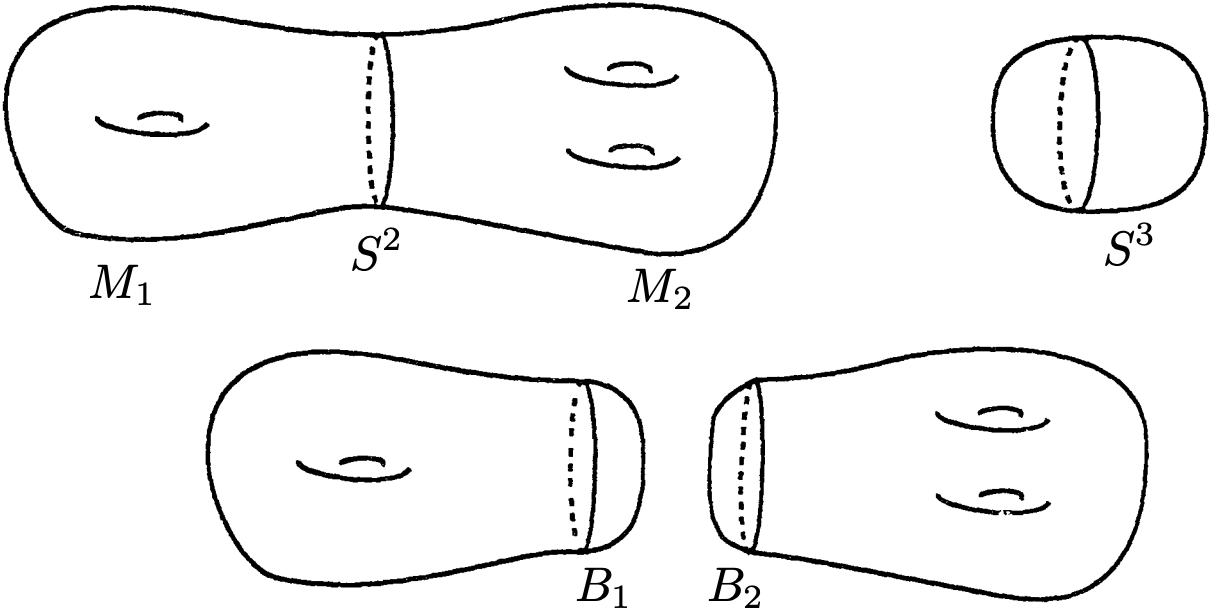
\includegraphics[width=0.85\textwidth]{figures/fig5_surgery.png}
  \caption{沿 $S^2$ 拆解 $M=M_1\#M_2$，并用 $S^3$ 的帽子把两块补圆。（原文 Figure 5，原文 p.31）}
  \label{fig:surgery}
\end{figure}

\paragraph{手术}
% 原文标题：Surgery.
前述讨论可以推广到包含威尔逊圈的情形；这会增大希尔伯特空间的维数，使线性代数更繁——人们会遇到 skein 关系等等——但总体图景基本相同。这一练习的副产品是：我们学会了如何显式计算 $S^3$ 中威尔逊圈的期望值。（这正是我们在 \S\ref{sec:3.4} 中未能兑现的一项任务。）手握 $S^3$ 上的期望值，人们就会梦想计算其他 3-流形
% ==== 原文 p.32 ====
$M\ne S^3$ 上的期望值。手术正是在这里登场：在任意 3-流形 $M$ 中给定一个纽结 $\gamma$，我们可以把 $\gamma$ 加粗成一根管 $T$，其拓扑是实心环面；从 $M$ 中挖去 $T$，对环面边界 $\partial T=T^2$ 施加一个巧妙选取的微分同胚，再把各块粘回去，就得到一个新的 3-流形 $\widetilde{M}$。三维拓扑学的一个基础结果是：任何 3-流形都可以由任何另一个经有限次沿嵌入纽结的手术得到。特别地，只要仔细考察手术对 $S^3$ 中威尔逊圈期望值做了什么，上述梦想就会实现。这正是 Witten 的做法。

% [Tutor Note: 含糊点] 「任何 3-流形可由任何另一个经有限次手术得到」= Lickorish–Wallace 定理（闭可定向 3-流形可由 S³ 沿链环作整系数 Dehn 手术得到）；原文未提 Kirby 移动与不变量良定义性。
\begin{yizhu}[含糊点]
「任何 3-流形都可以由任何另一个经有限次手术得到」是 Lickorish--Wallace 定理：任何闭可定向 3-流形都能由 $S^3$ 沿某个链环做整系数 Dehn 手术得到；原文的「从任意到任意」只是先回到 $S^3$ 再出来。要让 Witten 的论证闭合，还须说明手术描述的冗余（Kirby 移动）不改变结果，原文未提；而这一点恰是手术不变量良定义性的所在。
\end{yizhu}

事实上，这一论证与上面的论证几乎相同。从 $M=S^3$ 中挖去实心环面 $T$ 后，$T$ 与纽结补 $N=S^3\setminus T$ 的边界上各自驻留着一对典范对偶的希尔伯特空间 $\mathcal{H}_{T^2}$ 与 $\mathcal{H}_{\partial N}=\mathcal{H}^{*}_{T^2}$。$T$ 与 $N$ 上的路径积分分别给出向量 $|\psi\rangle\in\mathcal{H}_{T^2}$ 与 $|\chi\rangle\in\mathcal{H}_{\partial N}$；环面边界 $\partial T=T^2$ 上的微分同胚则在 $\mathcal{H}_{T^2}$ 上诱导一个线性变换 $K$，把 $|\psi\rangle\mapsto K|\psi\rangle$。于是新流形 $\widetilde{M}$ 上的路径积分通过算子 $K$ 与 $\mathcal{Z}(M)=\langle\chi|\psi\rangle$ 相联系：$\mathcal{Z}(\widetilde{M})=\langle\chi|K|\psi\rangle$。Witten 随后依据费林德的工作 [28] 描述亏格一的 CS 希尔伯特空间；他在 $T^2$ 上做一个模变换，靠手术从 $S^2\times S^1$ 得到 $S^3$，再借助亏格一的希尔伯特空间导出 $S^3$ 上 CS 配分函数的公式 \eqref{eq:3.32}。此后，整套程序再带源重复一遍。

% [Tutor Note: 易错点] H_{T²} 与 H_{∂N}=H*_{T²} 是同一亏格一空间的对偶写法（∂N=−T² 的定向负号已吸收进 *）；K 作用在 H_{T²} 上、夹在 ⟨χ| 与 |ψ⟩ 之间，误当作用于 H* 会给出转置。
\begin{yizhu}[易错点]
原文的记号要分清：$\mathcal{H}_{T^2}$ 是 $T$ 的边界上的希尔伯特空间，$\mathcal{H}_{\partial N}=\mathcal{H}^{*}_{T^2}$ 是纽结补的；二者本是同一个亏格一空间，星号只标对偶。$\partial T=T^2$ 与 $\partial N=-T^2$ 定向相反，这个负号已吸收进对偶里。$K$ 由 $\partial T$ 上的微分同胚诱导，作用在 $\mathcal{H}_{T^2}$ 上，故 $\langle\chi|K|\psi\rangle$ 中 $K$ 夹在对偶态与态之间；若误把 $K$ 当作作用于 $\mathcal{H}^{*}$，就得换成转置 $K^{T}$，配分函数随之改变。
\end{yizhu}

% =============================================================================
% 汇报（片段 s04b，对应原文 p.28–32）
% 覆盖：4.2 带源的量子化（p.28–29）、4.3 例：亏格零（p.29–31）、4.4 展望：手术与源（p.31–32）
% 编号公式：3 个 —— (4.5)(4.6)(4.7)，均以 \tag 锁定、顺序照原文
% 图：图 5（figures/fig5_surgery.png，width=0.85\textwidth，label=fig:surgery），位于 (4.7) 之后
% 脚注：原文脚注 9（p.29）已全译
% 译注：12 条 —— 易错点 5、含糊点 4、原文疑误 2、物理图像 1；每条前一行类型摘要注释
% 原文疑误（均照录并批注）：
%   1) p.30 毛球定理 => P^1 上无平坦联络、模空间为空：论证不成立（S^2 单连通，平凡丛平坦联络
%      模空间是单点 A=0）；结论「亏格零无标记时希尔伯特空间 1 维」不受影响。同页 nonwhere 应为 nowhere。
%   2) p.30 两标记点末句「R_2 ≠ R_1」应为「R_2 ≠ \bar R_1」。
% 存疑：无。图 4 的交叉引用用 \ref{fig:cut}（s04a 的 label），(2.27)/(3.32) 分别用 \eqref。
% 与 s01 一致：小节内的 run-in 小标题用 \paragraph{…} 且以半角句点收束；若 Lead 统一改为全角「。」请全局替换。
% =============================================================================
